% SSection Models
% Design (what)
% Reasoning (why)
% Implications on parallelism
% Allocation
% Figures of each each (design, allocation)

In this section, we evaluate the performance of different synchronization protocols in dxex.
We also compare to adevs~\cite{adevs}, currently one of the most efficient simulation kernels~\cite{DEVSSurvey,DEVStoneJournal}, to show that our modularity does not impede performance.
CPU time and memory usage is compared for both sequential and parallel simulation.

We start off with a comparison of sequential simulation, to show how adevs and dxex relate in this simple case.
For the parallel simulation benchmarks, results are presented for both conservative and optimistic synchronization.

For all benchmarks, results are well within a 5\% deviation of the average, such that only the average is used in the remainder of this section.
The same compilation flags were used for both adevs and dxex benchmarks (``\texttt{-O3 -flto}'').
To guarantee comparable results, no I/O was performed during benchmarks.
Before benchmarking, simulation traces were used to verify that adevs and dxex return exactly the same simulation results.
Benchmarks were performed using Linux, but our simulation tool works equally well on Windows and Mac.
The exact parameters for each benchmark can be found in the repository, as well as the data used in this paper. 

\subsection{Benchmarks}
We use three different benchmarks, which cover different aspects of the simulation kernel.

First, the \textit{Queue} model, based on the \textit{HI} model of DEVStone~\cite{DEVStone}, creates a chain of hierarchically nested atomic \textsf{DEVS} models.
A single generator pushes events into the queue, which are consumed by the processors after a fixed or random delay.
It takes two parameters: width and depth, which determine the width and depth of the hierarchy.
This benchmark shows how the complexity of the simulation kernel behaves for an increasing amount of atomic models, and an increasingly deep hierarchy.
An example for width and depth 2 is shown in Figure~\ref{fig:queue_model}.
	
Second, the \textit{PHOLD} model, presented by~\cite{PHOLD}, creates $n$ atomic models, where each model has exactly $n-1$ output ports.
Each atomic model is directly connected to every other atomic model.
After a random delay, an atomic model sends out an event to a randomly selected output port.
Output port selection happens in two phases: first it is decided whether the event should be sent to an atomic model at the same node.
Afterwards, a uniform selection is made between the remaining ports.
The model takes two parameter: the percentage of remote events, which determines the fraction of messages routed to other nodes, and the percentage of priority events. Priority events are events generated in a very short time after the previous event.
This benchmark shows how the simulation kernel behaves in the presence of many local or remote events and when the average time advance is larger than the lookahead in conservative simulation.
An example for four models, split over two nodes, is shown in Figure~\ref{fig:PHOLD_model}.
	
Third, the \textit{Interconnect} model, a merge of PHOLD~\cite{PHOLD} and the \textit{HI} model of DEVStone~\cite{DEVStone}, creates $n$ atomic models, where each model has exactly one output port.
Similar to PHOLD, all models are connected to one another, but all through the same port: every model receives each generated event.
The model takes one parameter: the number of models.
This benchmark investigates the complexity of event routing, and how the simulation kernel handles many simultaneous events.
An example for four models is shown in Figure~\ref{fig:interconnect_model}.

\begin{figure}
	\center
	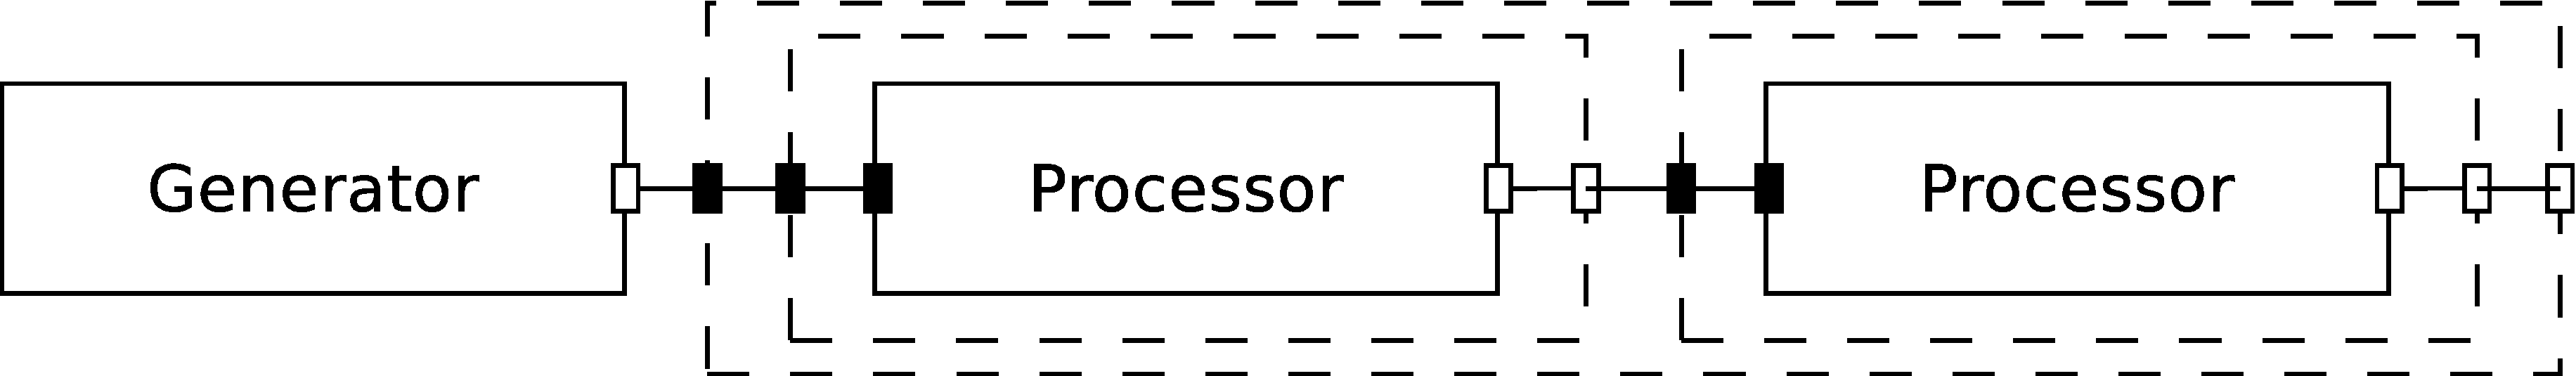
\includegraphics[width=\columnwidth]{fig/queue_model_fixed.pdf}
	\caption{Queue model for depth and width 2.}
	\label{fig:queue_model}
	
	\vspace{\betweenmodels}
	
	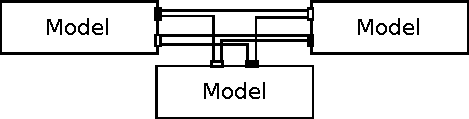
\includegraphics[width=\modelfraction\columnwidth]{fig/interconnect_model.pdf}
	\caption{Interconnect model for three models.}
	\label{fig:interconnect_model}
	
	\vspace{\betweenmodels}
	
	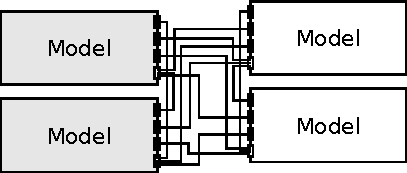
\includegraphics[width=\modelfraction\columnwidth]{fig/phold_model.pdf}
	\caption{PHOLD model for three models.}
	\label{fig:PHOLD_model}
\end{figure}
